\documentclass[12pt,a4paper,final]{article}
\usepackage[utf8]{inputenc}
\usepackage{amsmath}
\usepackage{amsfonts}
\usepackage{amssymb}
\usepackage{graphicx}
\usepackage{multicol}
\usepackage{quoting} 
\usepackage[LGR,T1]{fontenc}
\newcommand{\textgreek}[1]{\begingroup\fontencoding{LGR}\selectfont#1\endgroup}
\usepackage[a4paper,margin=1in]{geometry}
\usepackage{makecell}
\usepackage{tabularx}


\renewcommand{\thefootnote}{\Alph{footnote}}
\renewcommand{\textsuperscript}[1]{\ensuremath{^{\textbf{\scriptsize #1}}}}

\begin{document}

The NET’s uniquely transparent, accountable translation process has been crystalized in the most extensive set of Bible translators’ notes ever created. More than 60,000 notes highlight every major decision, outline alternative views, and explain difficult or nontraditional renderings. These are broken into: \textbf{sn} Study Notes, \textbf{tn} Translation Notes, and \textbf{tc} Text Critical notes (comparison of different manuscripts).

\section*{Daniel 4 (NET)}

\textsuperscript{1,(3:31)}\footnote{\textbf{sn} Beginning with 4:1, the verse numbers through 4:37 in the English Bible differ from the verse numbers in the Aramaic text (BHS), with 4:1 ET = 3:31 AT, 4:2 ET = 3:32 AT, 4:3 ET = 3:33 AT, 4:4 ET = 4:1 AT, etc., through 4:37 ET = 4:34 AT. Thus Dan 3:31–33 of the Aramaic text appears as Dan 4:1–3 in the English Bible, and the corresponding verses of ch. 4 differ accordingly. In spite of the division of the Aramaic text, a good case can be made that 3:31–33 AT (= 4:1–3 ET) is actually the introduction to ch. 4.}“King Nebuchadnezzar, to all peoples, nations, and language groups that live in all the land: Peace and prosperity! \textsuperscript{2}I am delighted to tell you about the signs and wonders that the most high God has done for me.\\ 
    \textsuperscript{3}“How great are his signs! \\
    How mighty are his wonders! \\
    His kingdom will last forever, \\ 
    and his authority continues from one generation to the next.” 

\subsubsection*{Nebuchadnezzar Dreams of a Tree Chopped Down}

\textsuperscript{4,(1)}\footnote{\textbf{sn} This verse marks the beginning of chap. 4 in the Aramaic text of Daniel (see the note on 4:1). The Greek OT (Septuagint) has the following addition: “In the eighteenth year of Nebuchadnezzar’s reign he said.” This date would suggest a link to the destruction of Jerusalem in 586 B.C.}I, Nebuchadnezzar, was relaxing in my home, living luxuriously\footnote{\textbf{tn} Aramaic “happy.”} in my palace.\textsuperscript{5}I saw a dream that frightened me badly. The things I imagined while lying on my bed—these visions of my mind—were terrifying me. \textsuperscript{6}So I issued an order for all the wise men of Babylon to be brought before me so that they could make known to me the interpretation of the dream. \textsuperscript{7}When the magicians, astrologers, wise men, and diviners entered, I recounted the dream for them. But they were unable to make known its interpretation to me. \textsuperscript{8}Later Daniel entered (whose name is Belteshazzar after the name of my god, and in whom there is a spirit of the holy gods). I recounted the dream for him as well, \textsuperscript{9}saying, “Belteshazzar, chief of the magicians, in whom I know there to be a spirit of the holy gods and whom no mystery baffles, consider my dream that I saw and set forth its interpretation! \textsuperscript{10}Here are the visions of my mind while I was on my bed. 
\begin{quotation}
\noindent While I was watching, \\
there was a tree in the middle of the land\footnote{\textbf{tn} Instead of “in the middle of the land,” some English versions render this phrase “a tree at the center of the earth” (NRSV); NAB, CEV “of the world”; NLT “in the middle of the earth.” The Hebrew phrase can have either meaning}. \\
It was enormously tall. \\
\textsuperscript{11}The tree grew large and strong.\\ 
Its top reached far into the sky; \\
it could be seen from the borders of all the land. \\
\textsuperscript{12}Its foliage was attractive and its fruit plentiful; \\
on it there was food enough for all. \\
Under it the wild animals used to seek shade, \\
and in its branches the birds of the sky used to nest. \\
All creatures\footnote{\textbf{tn} Aramaic “all flesh.”} used to feed themselves from it. \\
\textsuperscript{13}While I was watching in my mind’s visions on my bed, \\
a holy sentinel\footnote{\textbf{tn} Aramaic “a watcher and a holy one.” The expression is a hendiadys; so also in v. 23. This “watcher” is apparently an angel. The Greek OT (LXX) in fact has \textgreek{'aggelos} (angelos, “angel”) here. Theodotion simply transliterates the Aramaic word (’ir). The term is sometimes rendered “sentinel” (NAB) or “messenger” (NIV, NLT).} came down from heaven. \\
\textsuperscript{14}He called out loudly as follows: \\
‘Chop down the tree and lop off its branches! \\
Strip off its foliage \\
and scatter its fruit! \\
Let the animals flee from under it \\
and the birds from its branches! \\
\textsuperscript{15}But leave its taproot\footnote{\textbf{tn} Aramaic “the stock of its root.” So also v. 23. The implication here is that although the tree is chopped down, it is not killed. Its life-giving root is spared. The application to Nebuchadnezzar is obvious.} in the ground, \\
with a band of iron and bronze around it\footnote{\textbf{sn} The function of the band of iron and bronze is not entirely clear, but it may have had to do with preventing the splitting or further deterioration of the portion of the tree that was left after being chopped down. By application it would then refer to the preservation of Nebuchadnezzar’s life during the time of his insanity.} \\
surrounded by the grass of the field. \\
Let it become damp with the dew of the sky, \\
and let it live with the animals in the grass of the land. \\
\textsuperscript{16}Let his mind\footnote{\textbf{tn} Aramaic “its heart.” The metaphor of the tree begins to fade here and the reality behind the symbol (the king) begins to emerge.} be altered from that of a human being, \\
and let an animal’s mind be given to him, \\
and let seven periods of time go by for him. \\
\textsuperscript{17}This announcement is by the decree of the sentinels; \\
this decision is by the pronouncement of the holy ones, \\
so that those who are alive may understand \\
that the Most High has authority over human kingdoms, \\
and he bestows them on whomever he wishes. \\
He establishes over them even the lowliest of human beings.’ \\

\end{quotation}
\textsuperscript{18}“This is the dream that I, King Nebuchadnezzar, saw. Now you, Belteshazzar, declare its interpretation, for none of the wise men in my kingdom are able to make known to me the interpretation. But you can do so, for a spirit of the holy gods is in you.” 


\subsubsection*{Daniel Interprets Nebuchadnezzar’s Dream}

\textsuperscript{19}Then Daniel (whose name is also Belteshazzar) was upset for a brief time\footnote{\textbf{tn} Aramaic “about one hour.” The expression refers idiomatically to a brief period of time of undetermined length.}; his thoughts were alarming him. The king said, “Belteshazzar, don’t let the dream and its interpretation alarm you.” But Belteshazzar replied, “Sir, if only the dream were for your enemies and its interpretation applied to your adversaries! \textsuperscript{20}The tree that you saw that grew large and strong, whose top reached to the sky, and which could be seen in all the land, \textsuperscript{21}whose foliage was attractive and its fruit plentiful, and from which there was food available for all, under whose branches wild animals used to live, and in whose branches birds of the sky used to nest—\textsuperscript{22}it is you, O king! For you have become great and strong. Your greatness is such that it reaches to heaven, and your authority to the ends of the earth. \textsuperscript{23}As for the king seeing a holy sentinel coming down from heaven and saying, ‘Chop down the tree and destroy it, but leave its taproot in the ground, with a band of iron and bronze around it, surrounded by the grass of the field. Let it become damp with the dew of the sky, and let it live with the wild animals, until seven periods of time go by for him’—\textsuperscript{24}this is the interpretation, O king! It is the decision of the Most High that this has happened to my lord the king. \textsuperscript{25}You will be driven\footnote{\textbf{tn} The Aramaic indefinite active plural is used here like the English passive. So also in v. 28, 29, 32.} from human society, and you will live with the wild animals. You will be fed grass like oxen\footnote{\textbf{sn} Nebuchadnezzar’s insanity has features that are associated with the mental disorder known as boanthropy, in which the person so afflicted imagines himself to be an ox or a similar animal and behaves accordingly.}, and you will become damp with the dew of the sky. Seven periods of time will pass by for you, before you understand that the Most High is ruler over human kingdoms and gives them to whomever he wishes. \textsuperscript{26}They said to leave the taproot of the tree, for your kingdom will be restored to you when you come to understand that heaven\footnote{\textbf{sn} The reference to heaven here is a circumlocution for God. There was a tendency in Jewish contexts to avoid direct reference to God. Cf. the expression “kingdom of heaven” in the NT and such statements as “I have sinned against heaven and in your sight” (Luke 15:21).} rules. \textsuperscript{27}Therefore, O king, may my advice be pleasing to you. Break away from your sins by doing what is right, and from your iniquities by showing mercy to the poor. Perhaps your prosperity will be prolonged.”
 
\textsuperscript{28}Now all of this happened to King Nebuchadnezzar. \textsuperscript{29}After twelve months, he happened to be walking around on the battlements\footnote{\textbf{tn} The word “battlements” is not in the Hebrew text, but is supplied from context. Many English versions supply “roof” here (e.g., NAB, NASB, NIV, NRSV); cf. NLT “on the flat roof.”} of the royal palace of Babylon. \textsuperscript{30}The king uttered these words: “Is this not the great Babylon that I have built for a royal residence by my own mighty strength and for my majestic honor?” \textsuperscript{31}While these words were still on the king’s lips, a voice came down from heaven: “It is hereby announced to you, King Nebuchadnezzar, that your kingdom has been removed from you! \textsuperscript{32}You will be driven from human society, and you will live with the wild animals. You will be fed grass like oxen, and seven periods of time will pass by for you before you understand that the Most High is ruler over human kingdoms and gives them to whomever he wishes.” 
\textsuperscript{33}Now in that very moment this pronouncement about Nebuchadnezzar came true. He was driven from human society, he ate grass like oxen, and his body became damp with the dew of the sky, until his hair became long like an eagle’s feathers, and his nails like a bird’s claws\footnote{\textbf{tn} The words “feathers” and “claws” are not present in the Aramaic text, but have been added in the translation for clarity.}. 
\textsuperscript{34}But at the end of the appointed time I, Nebuchadnezzar, looked up toward heaven, and my sanity returned to me. 
\begin{quotation}

\noindent I extolled the Most High, \\
and I praised and glorified the one who lives forever.\\ 
For his authority is an everlasting authority, \\
and his kingdom extends from one generation to the next. \\
\textsuperscript{35}All the inhabitants of the earth are regarded as nothing. \\
He does as he wishes with the army of heaven \\
and with those who inhabit the earth. \\
No one slaps his hand\footnote{\textbf{tn} Aramaic “strikes against.”} \\
and says to him, ‘What have you done?’ \\

\end{quotation}
\textsuperscript{36}At that time my sanity returned to me. I was restored to the honor of my kingdom, and my splendor returned to me. My ministers and my nobles were seeking me out, and I was reinstated over my kingdom. I became even greater than before. \textsuperscript{37}Now I, Nebuchadnezzar, praise and exalt and glorify the King of heaven, for all his deeds are right and his ways are just. He is able to bring down those who live in pride. 

\newpage
\section*{Parallel Passages}
\begin{tabularx}{\linewidth}{lcX}
%\begin{tabular}{|p{2cm}|p{3cm}|p{10cm}|}
\hline 
\textbf{Daniel} & \textbf{NT} & \textbf{Verse(s)} \\ 
\hline 
4:2, 4:37 & John 4:48 & \textsuperscript{48}So Jesus said to him, “Unless you people see signs and wonders you will never believe!” \\ 
\hline 
4:12, 4:21 & Mark 4:30-32 & \textsuperscript{30}He also asked, “To what can we compare the kingdom of God, or what parable can we use to present it? \textsuperscript{31}It is like a mustard seed that when sown in the ground, even though it is the smallest of all the seeds in the ground—\textsuperscript{32}when it is sown, it grows up, becomes the greatest of all garden plants, and grows large branches so that the wild birds can nest in its shade.”  \\ 
\hline 
4:35 & Revelation 4:9-11 & \makecell[Xt]{\textsuperscript{9}And whenever the living creatures give glory, honor, and thanks to the one who sits on the throne, who lives forever and ever, \textsuperscript{10}the twenty-four elders throw themselves to the ground before the one who sits on the throne and worship the one who lives forever and ever, and they offer their crowns before his throne, saying: \\
    \textsuperscript{11}“You are worthy, our Lord and God, \\
    to receive glory and honor and power, \\
    since you created all things, \\
    and because of your will they existed and were created!" \\ 
}\\
\hline 
\end{tabularx}
%\end{tabular} 

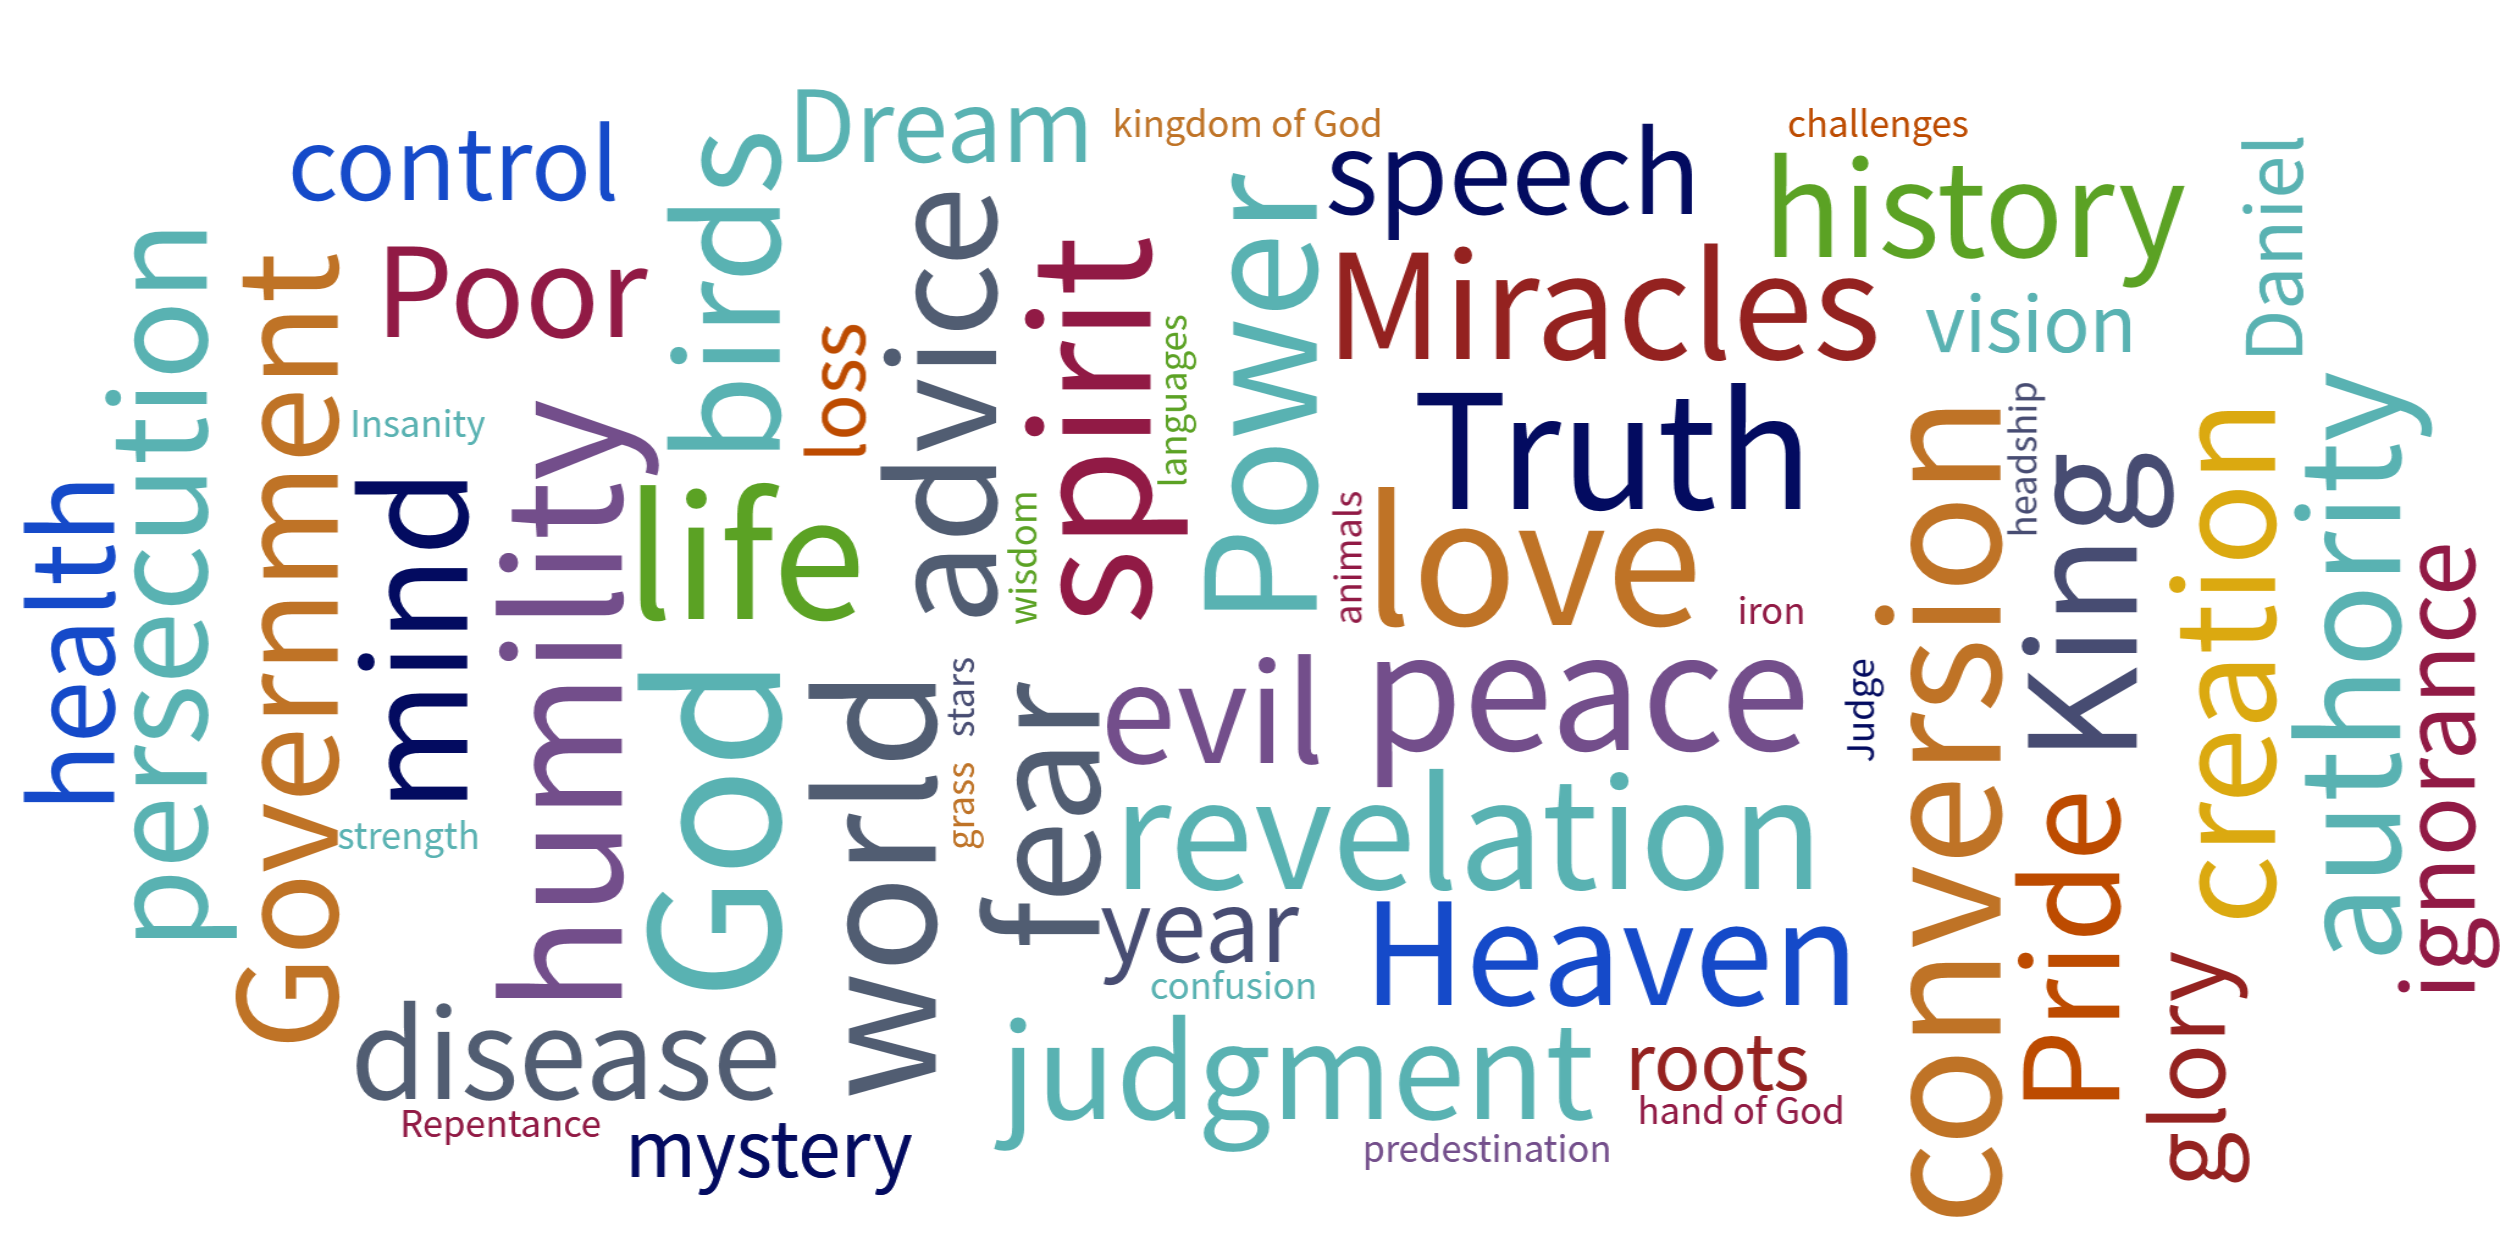
\includegraphics[width=\textwidth]{wordcloud.png} 
\end{document}

@book{Biblical Studies Press_2005,
title={The NET Bible First Edition; Bible. English. NET Bible.; The NET Bible},
publisher={Biblical Studies Press},
author={Biblical Studies Press},
year={2005},
pages={Da 4:4–37} }